\documentclass[12pt]{beamer}
\usepackage[utf8]{inputenc}
\usepackage{amsmath}
\usepackage{amsfonts}
\usepackage{amssymb,esint}
\usepackage{appendixnumberbeamer}
\usepackage{color}
\usepackage{verbatim} % comentarios
%\usepackage{beamerthemesplit}
%\usepackage{pb-diagram}
%\usepackage{ulem}
%\usepackage{overpic}
%\usepackage{tikz-cd}
\usepackage{graphicx}
\usepackage{subfigure}
\usepackage{pdfpages}
\usepackage{multicol}
\usepackage{forest}
\usepackage{stmaryrd}
\usepackage{tikz}
\usepackage{tikz-cd}
\usepackage{mathtools}
%\usepackage{caption}
%\usepackage{subcaption}
\usepackage[english,spanish]{babel}
\usepackage[duration=15,enduserslide=14]{pdfpcnotes}
\usepackage{movie15}
\mode<presentation>

\graphicspath{{./img/}}

%%%%%%%%%%%%%%%% Tikz %%%%%%%%%%%%%%

\usetikzlibrary{arrows, matrix}

%%%%%%%%%%%%%%%% Open with `pdfpc` %%%%%%%%%%%%%%

\setbeamertemplate{navigation symbols}{}

\usetheme{Warsaw}

\setbeamercovered{transparent}

%\setbeameroption{show notes on second screen=right}

\setbeamercolor{mycolor}{fg=white,bg=black}

\defbeamertemplate*{footline}{shadow theme}{%
\leavevmode%
\hbox{\begin{beamercolorbox}[wd=.5\paperwidth,ht=2.5ex,dp=1.125ex,leftskip=.3cm plus1fil,rightskip=.3cm]{author in head/foot}%
    \usebeamerfont{author in head/foot}\hfill\insertshortauthor
\end{beamercolorbox}%
\begin{beamercolorbox}[wd=.43\paperwidth,ht=2.5ex,dp=1.125ex,leftskip=.3cm,rightskip=.3cm plus1fil]{title in head/foot}%
    \usebeamerfont{title in head/foot}\hfill%
\end{beamercolorbox}%
\begin{beamercolorbox}[wd=.07\paperwidth,ht=2.5ex,dp=1.125ex,leftskip=.1cm,rightskip=.1cm plus1fil]{mycolor}%
\hfill\insertframenumber\,/\,\inserttotalframenumber
\end{beamercolorbox}}%
\vskip0pt%
}

%%%%%%%%%%%%%%%%%%%%%%%%%%%%%%%%%%%%%%%%%%%%%%%%

%%%%% NUMEROS %%%%%%%%%%%%%%%%%%%%%%%%%%%%%%%%%%%%%%%

\newcommand{\e}{\mathrm{e}}
\newcommand{\ii}{\mathrm{i}}
\renewcommand{\r}{\mathbf{r}}
\renewcommand{\d}{\mathrm{d}}
\newcommand{\al}{&\,}

\renewcommand{\bf}[1]{{\boldsymbol{#1}}}

%%%%% CONJUNTOS NUMERICOS %%%%%%%%%%%%%%%%%%%%%%%%%%%

\newcommand{\C}{\ensuremath{\mathbb{C}}}
\newcommand{\N}{\ensuremath{\mathbb{N}}}
\newcommand{\Q}{\ensuremath{\mathbb{Q}}}
\newcommand{\R}{\ensuremath{\mathbb{R}}}
\newcommand{\T}{\ensuremath{\mathbb{\zeta}}}
\newcommand{\Z}{\ensuremath{\mathbb{Z}}}

%%%%% FUNCIONES %%%%%%%%%%%%%%%%%%%%%%%%%%%%%%%%%%%%%

\renewcommand{\Re}[1]{\ensuremath{\mathrm{Re}\pa{ #1 }}}
\renewcommand{\Im}[1]{\ensuremath{\mathrm{Im}\pa{ #1 }}}
\renewcommand{\ker}[1]{\ensuremath{\mathrm{Ker}\pa{ #1 }}}
\newcommand{\ran}[1]{\ensuremath{\mathrm{Ran}\pa{ #1 }}}
\newcommand{\inc}{\ensuremath{\iota}}
\newcommand{\sig}[1]{\ensuremath{\mathrm{sgn}\pa{ #1 }}}
\newcommand{\sop}[1]{\ensuremath{\mathrm{sop}\pa{ #1 }}}
\newcommand{\tr}[1]{\ensuremath{\mathrm{tr}\pa{ #1 }}}
\newcommand*{\bigtimes}{\mathop{\raisebox{-.5ex}{\hbox{\huge{$\times$}}}}}

%%%%% LLAVES %%%%%%%%%%%%%%%%%%%%%%%%%%%%%%%%%%%%%%%%

\newcommand{\abs}[1]{\ensuremath{\left| #1 \right|}}
\newcommand{\norm}[1]{\ensuremath{\left\| #1 \right\|}}
\newcommand{\pa}[1]{\ensuremath{\left( #1 \right)}}
\newcommand{\pro}[2]{\ensuremath{\pa{ #1,#2 }}}
\newcommand{\set}[1]{\ensuremath{\left\{ #1 \right\}}}

%%%%% ESPACIOS VECTORIALES %%%%%%%%%%%%%%%%%%%%%%%%%%%%%

\newcommand{\Rn}[1][n]{\ensuremath{\R^{#1}}}
\newcommand{\Cn}[1][n]{\ensuremath{\C^{#1}}}

%%%%% ESPACIOS FUNCIONALES %%%%%%%%%%%%%%%%%%%%%%%%%%%%%

\newcommand{\sch}[1][n]{\ensuremath{\mathcal{S}\pa{\Rn[#1]}}}
\newcommand{\lp}[2]{\ensuremath{L^{#1}\pa{\Rn[#2]}}}
\newcommand{\lpw}[2]{\ensuremath{L^{#1,w}\pa{\Rn[#2]}}}
\newcommand{\sob}[2]{\ensuremath{H^{#1}\pa{\Rn[#2]}}}
\newcommand{\hil}{\ensuremath{\mathrm{H}}}

%%%%% Variables %%%%%%%%%%%%%%%%%%%%%%%%%%%%%

\renewcommand{\b}{\mathnormal{b}}
\newcommand{\f}{\mathnormal{f}}
\newcommand{\n}{\mathnormal{n}}
\newcommand{\p}{\mathnormal{p}}
\newcommand{\x}{\mathnormal{x}}
\newcommand{\y}{\mathnormal{y}}

\newcommand{\new}{\mathnormal{new}}
\newcommand{\meas}{\mathnormal{meas}}

% ------ Macros varios -------------
\newcommand{\lSV}{ \ensuremath{\lambda_{q}} }
\newcommand{\lR}{ \ensuremath{\lambda_{\rho}} }
\newcommand{\lRp}{ \ensuremath{\lambda_{\rho}^{pure}} }
\newcommand{\lRcv}{ \ensuremath{\lambda_{\rho}^{cbv}} }
\newcommand{\lRo}{ \ensuremath{\lambda_{\rho}^o} }

\newcommand{\tSV}{\ensuremath{ T_{q} } }
\newcommand{\tR}{\ensuremath{ T_{\rho} } }
\newcommand{\tRp}{\ensuremath{ T_{\rho}^\# } }
\newcommand{\tRo}{\ensuremath{ T_{\rho}^o } }

\newcommand{\vSV}{\ensuremath{ V_{q} } }
\newcommand{\vR}{\ensuremath{ V_{\rho} } }
\newcommand{\vRo}{\ensuremath{ V_{\rho}^o } }

\newcommand{\treeR}[1]{ tree_\rho(#1) }
\newcommand{\treeSV}[1]{ tree_q(#1) }
\newcommand{\collectR}[1]{ collect^{=}(#1) }
\newcommand{\collectSV}[1]{ collect^\stateEq(#1) }

\newcommand{\rp}[1]{ \llparenthesis #1 \rrparenthesis }
\newcommand{\chooseP}[1]{ choose(#1) }
\newcommand{\pureP}[1]{ pure\_terms(#1) }

\renewcommand{\rq}{*}
\newcommand{\rqt}{*}
\newcommand{\qr}{\vartriangle}
\newcommand{\qrt}{\vartriangle}

\newcommand{\tocbv}[1]{\llbracket #1 \rrbracket}
\newcommand{\ifte}[3]{\ensuremath{\; \text{if} \; #1 \; \text{then} \; #2 \;
                                     \text{else} \; #3 \;}}
\newcommand{\letin}[3]{\ensuremath{\; \text{let} \; #1 \; = \; #2 \;
                                     \text{in} \; #3 \;}}
\newcommand{\letcase}[3]{\ensuremath{\; \text{letcase} \; #1 \; = \; #2 \;
                                     \text{in} \; #3 \;}}
\newcommand{\letcaseo}[3]{\ensuremath{\; \text{letcase}^o \; #1 \; = \; #2 \;
                                     \text{in} \; #3 \;}}
\newcommand{\letcaseq}[2]{\ensuremath{\; \text{case} \; #1 \;
                                     \text{of} \; #2 \;}}
\newcommand{\decompose}[1]{\ensuremath{\; \text{decompose}(#1)}}
\newcommand{\state}[1]{\ensuremath{\; \text{fst}(#1)}}
\newcommand{\linker}[1]{\ensuremath{\; \text{snd}(#1)}}
\newcommand{\term}[1]{\ensuremath{\; \text{trd}(#1)}}
\newcommand{\stateEq}{\approx}
\newcommand{\probEq}{\approx_{prob}}

\newcommand{\oarrow}{ \rightsquigarrow }

\newcommand{\ketZero}{
    \begin{pmatrix}
        1 \\
        0
    \end{pmatrix}
}

\newcommand{\ketOne}{
    \begin{pmatrix}
        0 \\
        1
    \end{pmatrix}
}

\newcommand{\densityZero}{
    \begin{pmatrix}
        1 & 0 \\
        0 & 0
    \end{pmatrix}
}

\newcommand{\densityOne}{
    \begin{pmatrix}
        0 & 0 \\
        0 & 1
    \end{pmatrix}
}

\newcommand{\densityPlus}{
    \begin{pmatrix}
        \frac{1}{2} & \frac{1}{2} \\
        \frac{1}{2} & \frac{1}{2}
    \end{pmatrix}
}

\newcommand{\densityMinus}{
    \begin{pmatrix}
        \frac{1}{2} & -\frac{1}{2} \\
        -\frac{1}{2} & \frac{1}{2}
    \end{pmatrix}
}

\newcommand{\densityMixZO}{
    \begin{pmatrix}
        \frac{1}{2} & 0 \\
        0 & \frac{1}{2}
    \end{pmatrix}
}

\newcommand{\questeq}{\stackrel{?}{=}}

\newcommand{\braket}[2]{\langle#1|#2\rangle}
\newcommand{\ketbra}[2]{|{#1}{\times}{#2}|}
\newcommand{\bra}[1]{\langle#1|}
\newcommand{\ket}[1]{|#1\rangle}

%%%%%%%%%%%%%%%%%%%%%%%%%%%%%%%%%%%%%

\newcommand{\alComment}[1]{
  \text{\phantom{(#1)}} \tag*{#1}
}


%%%%%%%%%%%%%%%%%%%%% Cosas de BMC

\newcommand{\SAT}[1]{\llbracket#1\rrbracket_{k}}

\newcommand{\loopSAT}[1]{\prescript{}{l}{\SAT{#1}}}

\newcommand{\tSAT}{\SAT{M,f}}

\title[Título]{Título}

\author[Borgna, Freund, Scherman, Singer]{Agustín Borgna, Teodoro Freund, Jonathan Scherman, Jessica Singer}

\institute[UBA]{Universidad de Buenos Aires}

\date{December 21,  2018}

\AtBeginSection[]{\frame[noframenumbering]{\tableofcontents[current]}}

\begin{document}

\maketitle

\begin{frame}[noframenumbering]
\tableofcontents

\end{frame}

%%%%%%%%%%%%%%%%%%%%%%%%%%%%%%%%%%%%%%%%%%%%%%%%%%%%%%%%%%%%%%%%%%%%%%%%%%%%%%%%%
\section{Introduccion y Motivacion}

\frame{
\frametitle{Introduccion y Motivacion}

\begin{itemize}
    \item La tomografía computada es una tecnologia que permite conseguir una imagen de un corte (o seccion) del cuerpo.
    
    \item Distinta disposicion de los rayos dan distintos resultados y si uno quisiese encontrar la mejor topologia, deberia conducir estudios de rayos x (caros) en seres humanos (peligrosos), de aqui sale la motivacion de poder simular este proceso.
\end{itemize}

\pnote{1. Atravesando el objeto con rayos y midiendo la intensidad y el tiempo con el que llegan}

}

%%%%%%%%%%%%%%%%%%%%%%%%%%%%%%%%%%%%%%%%%%%%%%%%%%%%%%%%%%%%%%%%%%%%%%%%%%%%%%%%%

\section{Simulación}

\subsection{Generando los rayos}

\frame{
\frametitle{Tipos de rayos}

\begin{figure}[H]
\centering
  \begin{tabular}{@{}ccc@{}}
      Axiales & Laterales & Random\\
    
\includegraphics[width=.3\textwidth]{exp-anal/raysAxial100-checkboard.png} &
    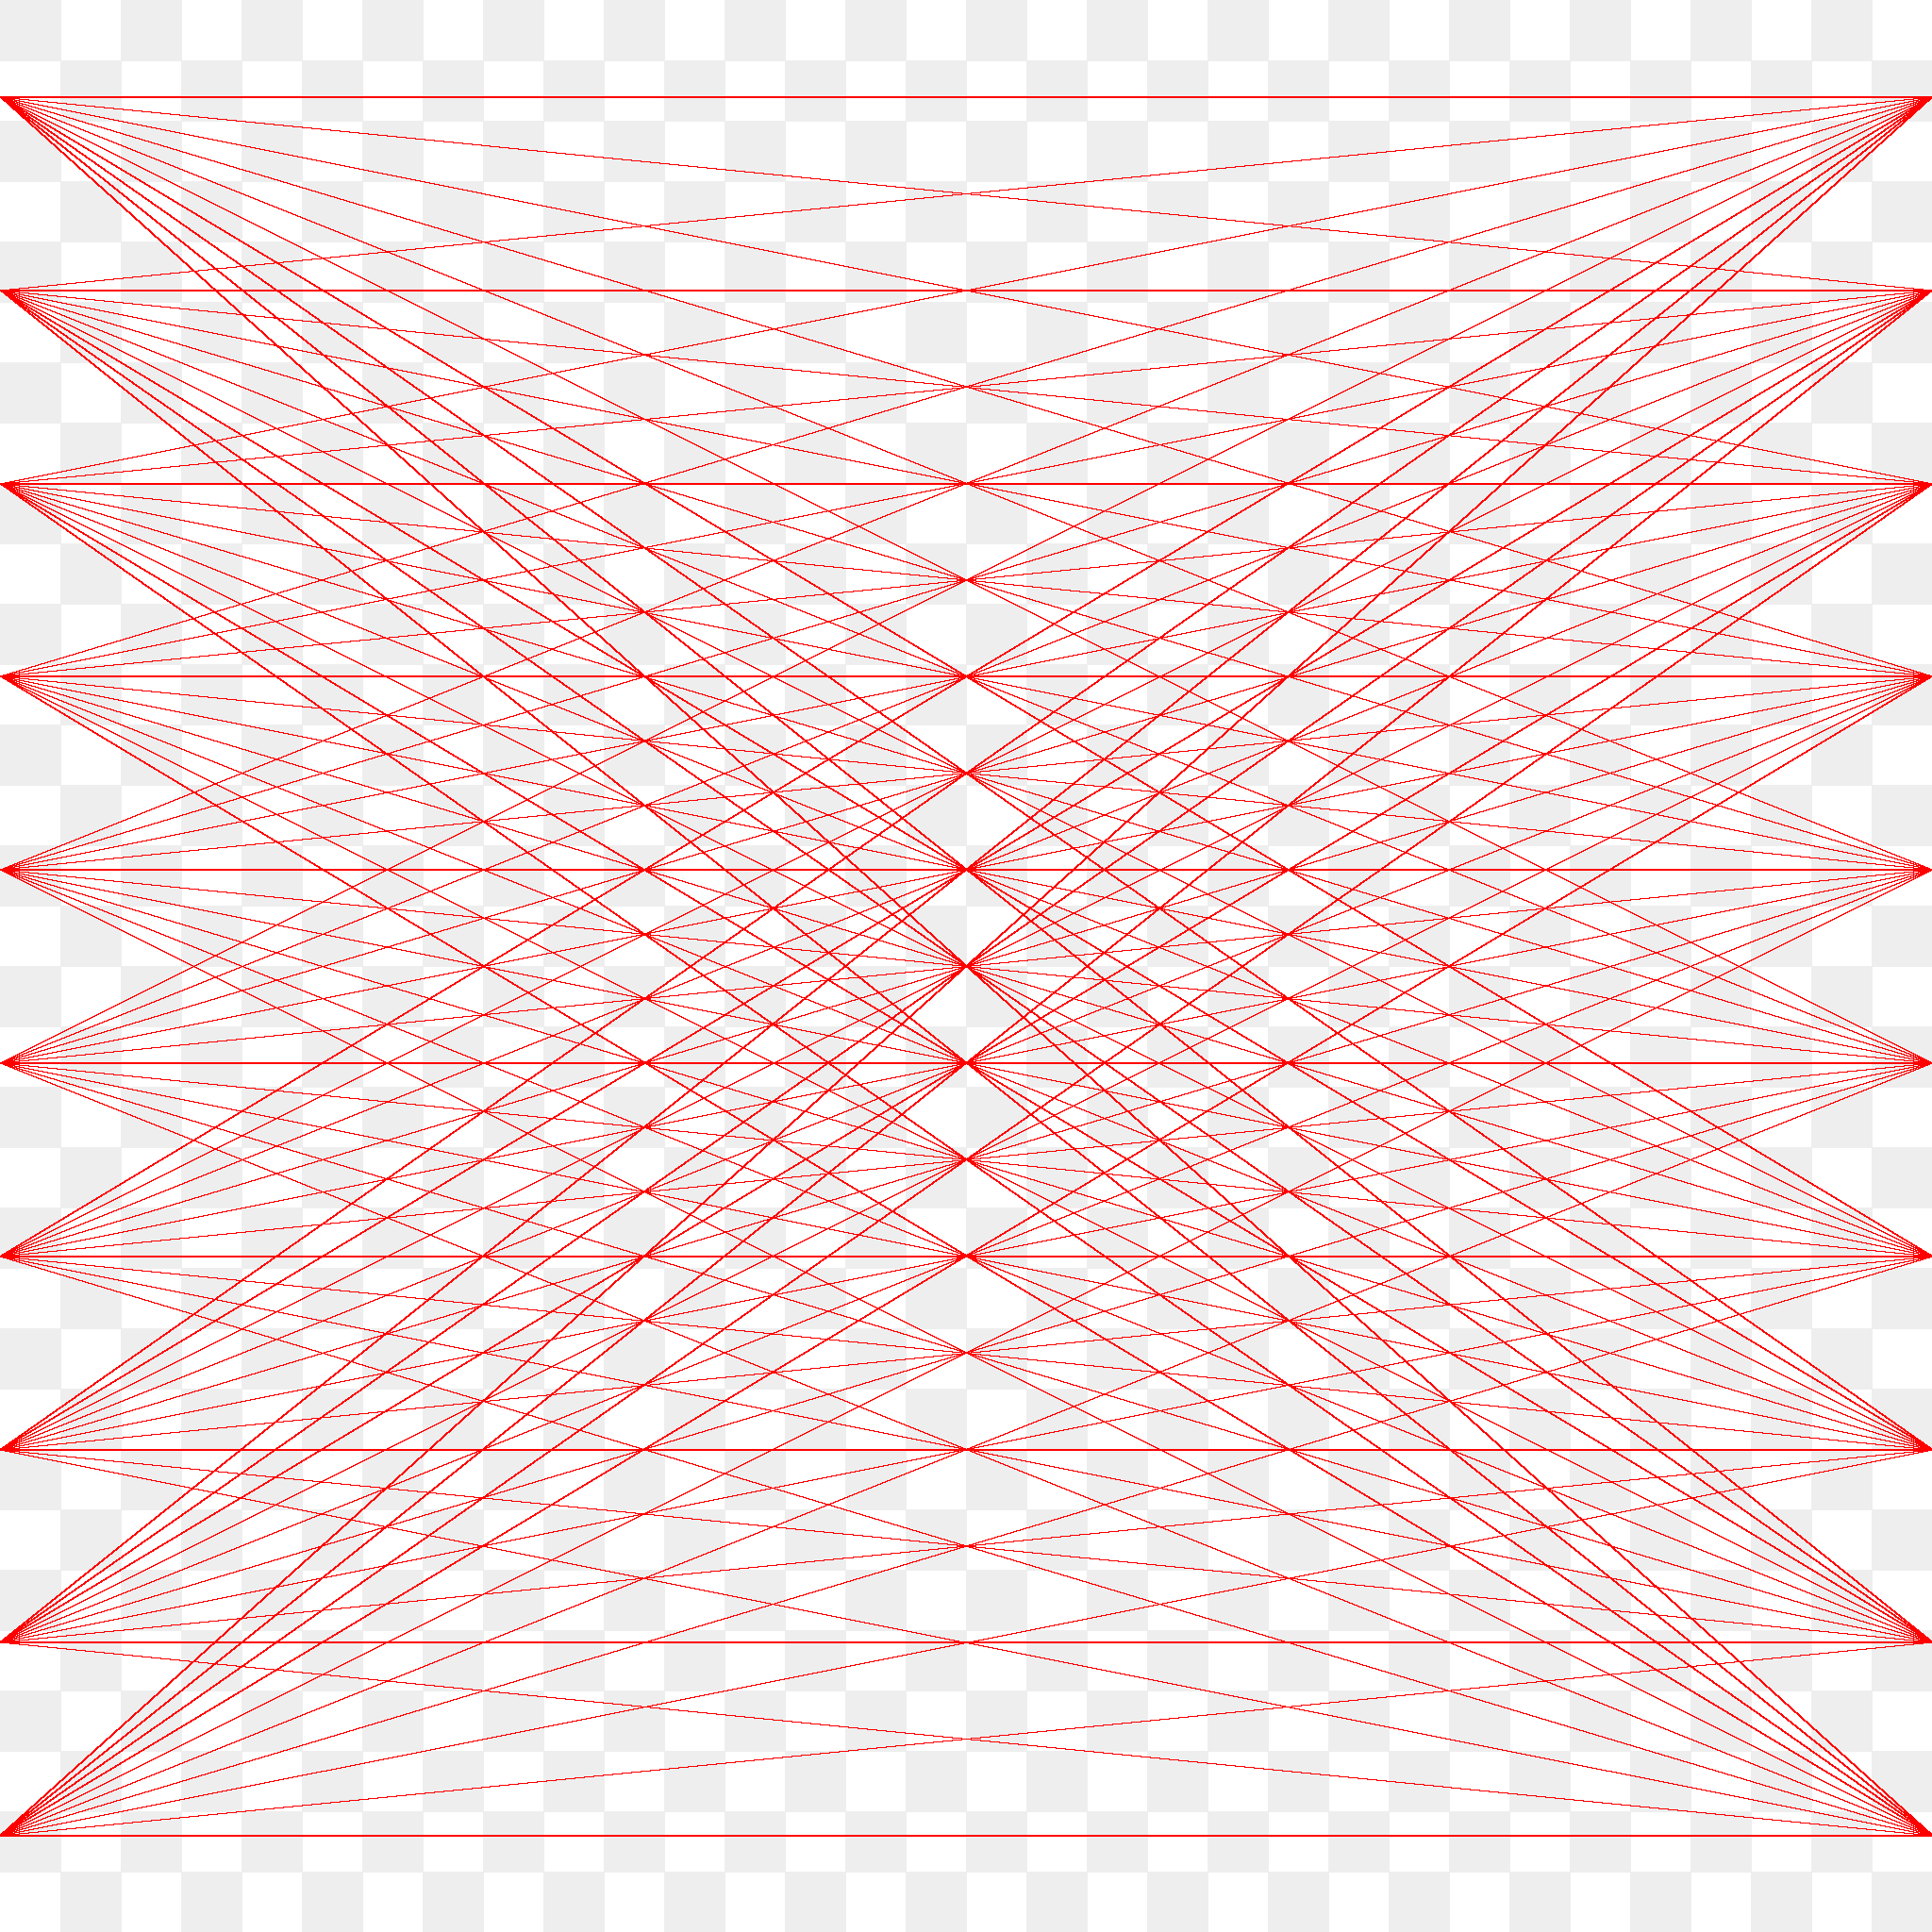
\includegraphics[width=.3\textwidth]{img/exp-anal/raysSides100-checkboard.png} &
    
\includegraphics[width=.3\textwidth]{exp-anal/raysRandom100-checkboard.png} & \\
  \end{tabular}
\end{figure}

\vspace*{4em}

    % \pnote{- Así se pueden agregar notas para la presentación}
}

\subsection{Vectores de incidencia}

\frame{
\frametitle{Calculando vectores de incidencia}


    \vspace*{4em}

  \begin{tabular}{@{}cc@{}}
      Bresenham & Xiaolin Wu \\
      
    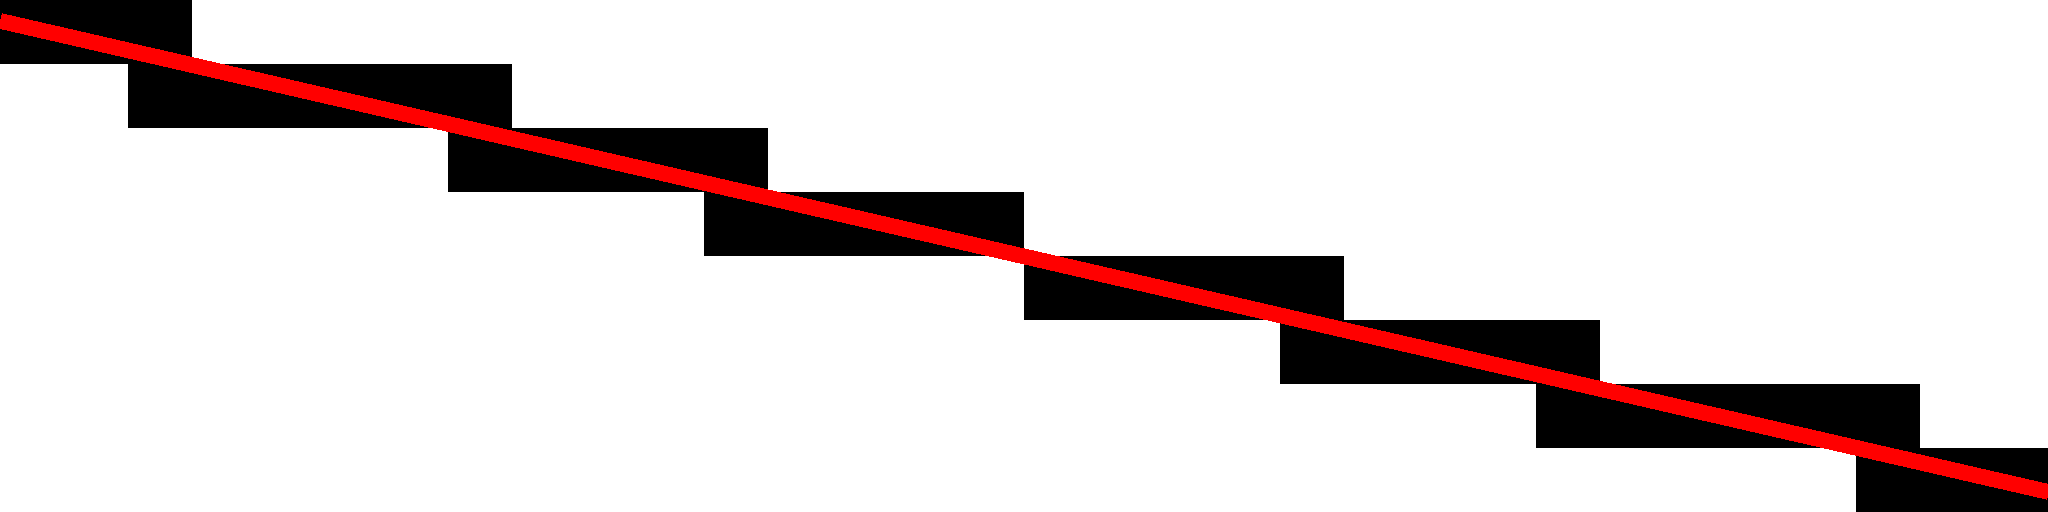
\includegraphics[width=.5\textwidth]{img/line-aliasing/rayDiagBres.png} &
    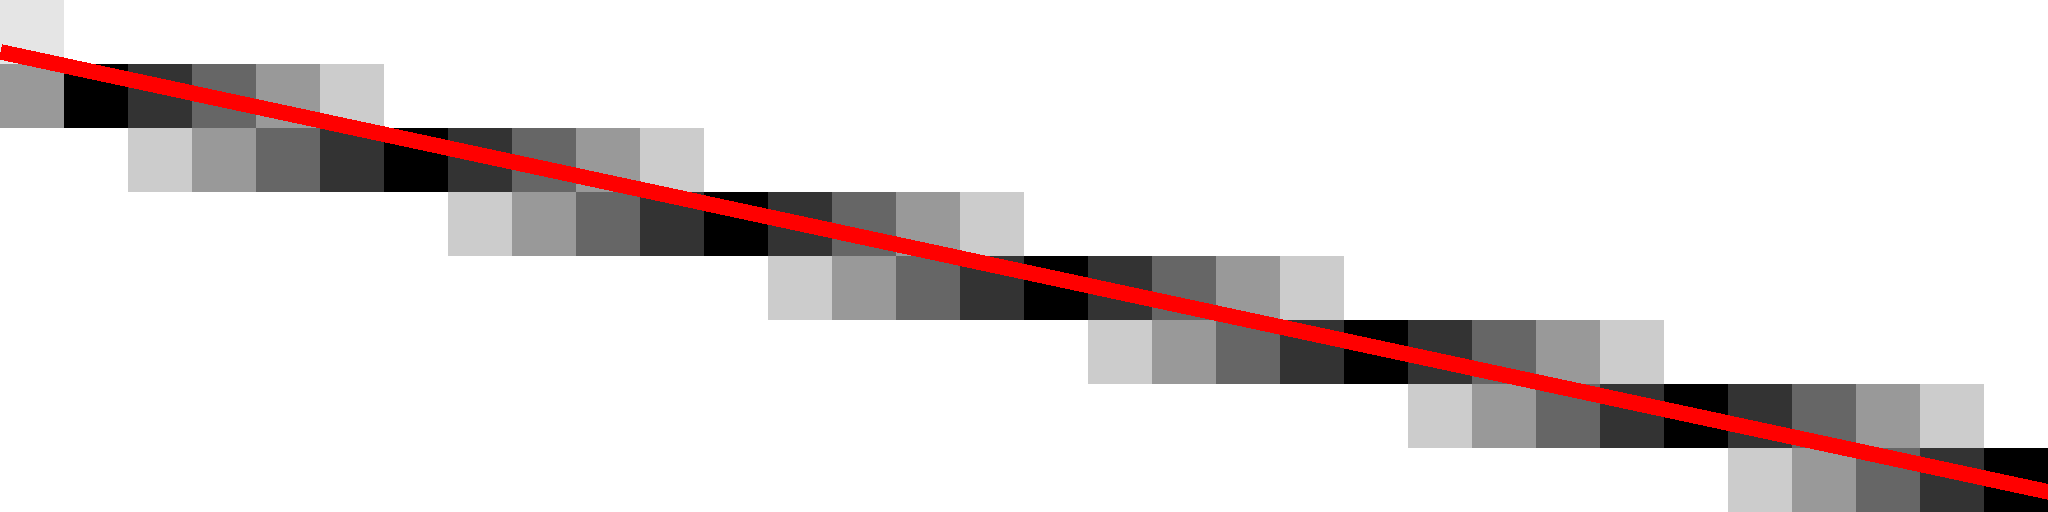
\includegraphics[width=.5\textwidth]{img/line-aliasing/rayDiag.png} & \\

  \end{tabular}
  
    \vspace*{4em}
    \hyperlink{frame:rayos-heatmap}{\beamergotobutton{Heatmaps}}
    
    % \includemovie{1cm}{1cm}{img/LineXiaolinWu.gif}

    \pnote{- Usamos Bresenham y Xiaolin Wu (backup).}
}


%%%%%%%%%%%%%%%%%%%%%%%%%%%%%%%%%%%%%%%%%%%%%%%%%%%%%%%%%%%%%%%%%%%%%%%%%%%%%%%%%
\section{Experimentación}

\frame{
\frametitle{Scripts para mediciones}

\begin{itemize}
    \item Generamos un script que redimensiona la imagen y la inyecta en el programa
    \item Cacheamos datos para acelerar la experimentación
    \item Medimos para cada ejecución su PSNR y tiempos.
\end{itemize}
}

\subsection{Variando cant. y tipo de rayos}

\frame{
\frametitle{Outputs usando tomo2.png}


\begin{figure}[H]
\centering
  \begin{tabular}{@{}cccc@{}}
      original & axial rays & side rays & random rays \\
      
    
\includegraphics[width=.2\textwidth]{img/exp-variando-rayos/tomo2-32-original.png} &
    
\includegraphics[width=.2\textwidth]{exp-variando-rayos/tomo2-32-0-19100-0-0-1-00001-1-1.png} &
    
\includegraphics[width=.2\textwidth]{exp-variando-rayos/tomo2-32-1-19100-0-0-1-00001-1-1.png} &
    
\includegraphics[width=.2\textwidth]{exp-variando-rayos/tomo2-32-2-19100-0-0-1-00001-1-1.png} & \\

  \end{tabular}
  
  
    \pnote{- en tomo2.png de 32x32}
    \pnote{- 20k rayos}
    \pnote{- error gaussiano con desvío estandar de 0.1}
    \pnote{- alpha=0.0001}
\end{figure}
}

%%%%%%%%%%%%%%%%%%%%%%%%%%%%%%%%%%%%%%%%%%%%%%%%%%%%%%%%%%%%%%%%%%%%%%%%%%%%%%%%%

\frame{
\frametitle{Tiempos y PSNR}

    \pnote{- en tomo2.png de 32x32}
    \pnote{- variando cant. rayos de 100 a 2000 (saltos de a 1000)}
    \pnote{- error gaussiano con desvío estandar de 0.1}
    \pnote{- alpha=0.0001}

\begin{figure}[H]
\centering
  \begin{tabular}{@{}cc@{}}
    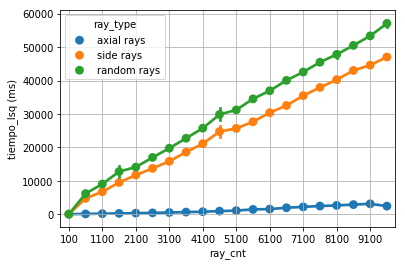
\includegraphics[width=.4\textwidth]{exp-variando-rayos/tiempos-variando-rayos-tomo2.png} &
    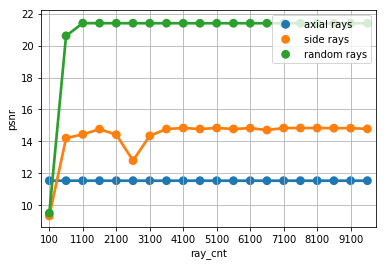
\includegraphics[width=.4\textwidth]{exp-variando-rayos/psnr-variando-rayos-tomo2.png} & 
    Tiempos & PSNR
  \end{tabular}
\end{figure}

}

%%%%%%%%%%%%%%%%%%%%%%%%%%%%%%%%%%%%%%%%%%%%%%%%%%%%%%%%%%%%%%%%%%%%%%%%%%%%%%%%%
\subsection{Variando ruido}

\frame{
\frametitle{Análisis de ruido}

\begin{figure}[H]
\centering
  \begin{tabular}{@{}cc@{}}
    \raisebox{0.5in}{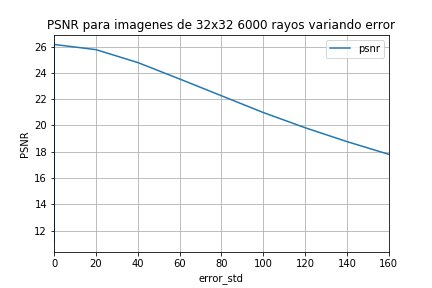
\includegraphics[width=.5\textwidth]{img/exp-error/exp-error.png}} &
    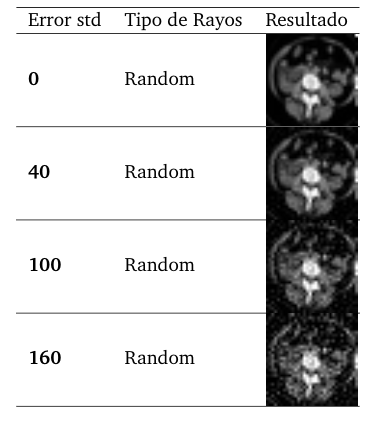
\includegraphics[width=.5\textwidth]{img/exp-error/tab1-posta.png}& 
  \end{tabular}
\end{figure}

}

%%%%%%%%%%%%%%%%%%%%%%%%%%%%%%%%%%%%%%%%%%%%%%%%%%%%%%%%%%%%%%%%%%%%%%%%%%%%%%%%%
\subsection{Variando valores singulares}

\frame{
\frametitle{Resultados variando valores singulares}


\begin{figure}[H]
\centering
  \begin{tabular}{@{}cc@{}}
    \raisebox{0.5in}{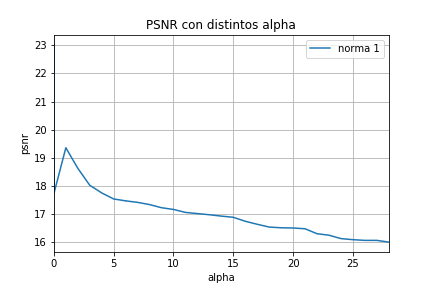
\includegraphics[width=.5\textwidth]{img/exp-variando-alpha/exp-distintos-alpha.png}} &
    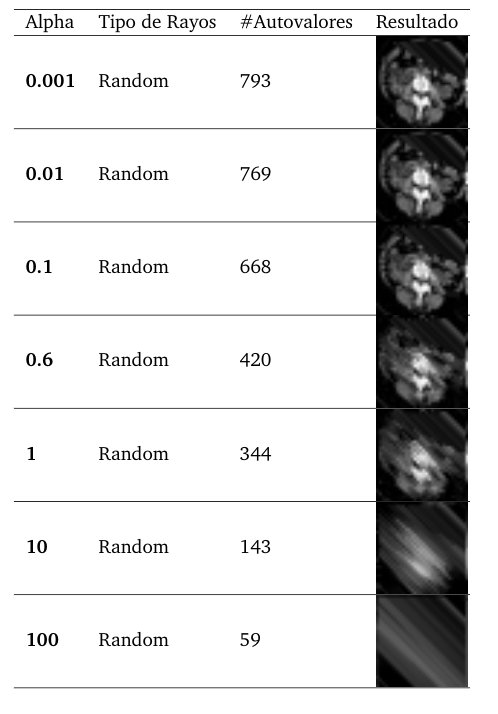
\includegraphics[width=.4\textwidth]{img/exp-variando-alpha/tab2.png}& 
  \end{tabular}
\end{figure}

}



%%%%%%%%%%%%%%%%%%%%%%%%%%%%%%%%%%%%%%%%%%%%%%%%%%%%%%%%%%%%%%%%%%%%%%%%%%%%%%%%%
\subsection{Experimentando con nro. de condición}

\frame{
\frametitle{Nro. de condición}


\begin{figure}[H]
\centering
  \begin{tabular}{@{}cc@{}}
    {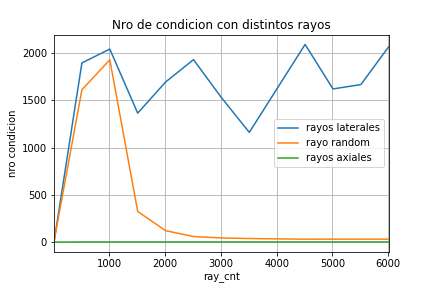
\includegraphics[width=.5\textwidth]{img/exp-nro-cond/exp-nro-cond-cond.png}} &
    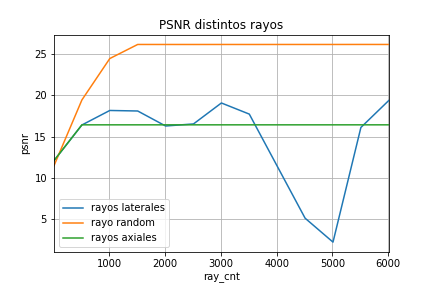
\includegraphics[width=.5\textwidth]{img/exp-nro-cond/exp-nro-cond.png}& 
  \end{tabular}
\end{figure}

}

\frame{
\frametitle{Nro. de condición}



\begin{figure}[H]%
    \centering
    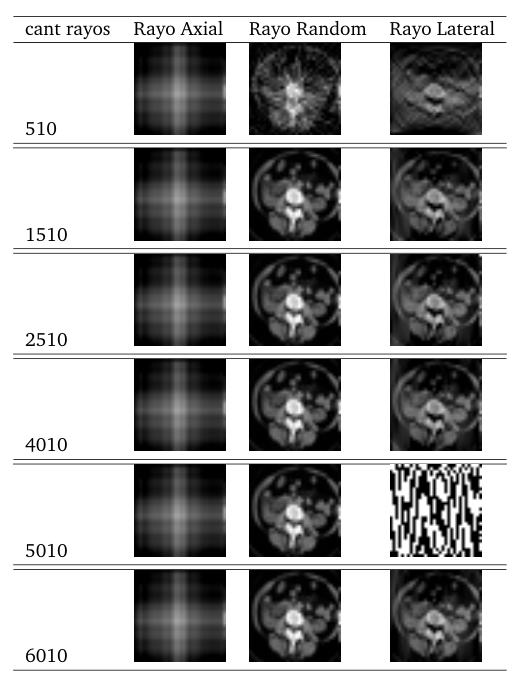
\includegraphics[width=.4\textwidth]{img/exp-nro-cond/tab3.png}%

\end{figure}

}





%%%%%%%%%%%%%%%%%%%%%%%%%%%%%%%%%%%%%%%%%%%%%%%%%%%%%%%%%%%%%%%%%%%%%%%%%%%%%%%%%

\section{Conclusiones y Trabajo Futuro}

\frame{

\frametitle{Conclusiones}

\begin{itemize}
    \item Tener una forma de simular este proceso (caro) nos permitió experimentar exhaustivamente.
    
    \item Tomar más o menos valores singulares para la descomposición SVD nos permite analizar un trade off entre velocidad de procesamiento y calidad del resultado.
\end{itemize}

\pnote{1. Se entendio la motivacion inicial. Un sistema más complejo podría ser muy útil para distintos investigadores.}
\pnote{2. Comparar con el tp anterior y bla.}


}

\frame{
\frametitle{Trabajo Futuro}


\begin{itemize}
    \item Rayos más complejos;
    \item otras formas de resolver CML;
    \pause
    \item rendir el final.
\end{itemize}
\pnote{1. no rectas, algun algoritmo que los mejore (busques local)}
\pnote{2. QR}
}

%%%%%%%%%%%%%%%%%%%%%%%%%%%%%%%%%%%%%%%%%%%%%%%%%%%%%%%%%%%%%%%%%%%%%%%%%%%%%%%%%

\section{Referencias}

\frame{
\bibitem{salomon}
\small
Salomon, David. (2007). Data Compression: \textit{The Complete Reference}. 281.

\bibitem{xiaolinWu}
Wu, Xiaolin (1991). "Fast Anti-Aliased Circle Generation". In James Arvo. Graphics Gems II. San Francisco: Morgan Kaufmann. pp. 446–450. ISBN 0-12-064480-0.

\bibitem{Condicion}
Belsley, David A.; Kuh, Edwin; Welsch, Roy E. (1980). "The Condition Number". Regression Diagnostics: Identifying Influential Data and Sources of Collinearity. New York: John Wiley & Sons.

\bibitem{SVD}
sepwww.stanford.edu/public/docs/sep73/ray1/paper\_html/node3.html

\pnote{1. Sirvio para tener valores ESPERADOS de PSNR}
\pnote{    2. El algoritmo loco}
\pnote{3. cosas de numero de condicion}
\pnote{4. SVD reducida}
}



%%%%%%%%%%%%%%%%%%%%%%%%%%%%%%%%%%%%%%%%%%%%%%%%%%%%%%%%%%%%%%%%%%%%%%%%%%%%%%%%%

\appendix
% start backup slides here

% Estas frames quedan fuera de la numeración y del índice
%\frame{
%\frametitle{asd2}
%}

\frame{
\label{frame:rayos-heatmap}
\frametitle{Heatmap de rayos}

\begin{figure}[H]
\centering
  \begin{tabular}{@{}ccc@{}}
      Axiales & Laterales & Random\\
    
\includegraphics[width=.3\textwidth]{exp-anal/raysAxial100-heatmap.png} &
    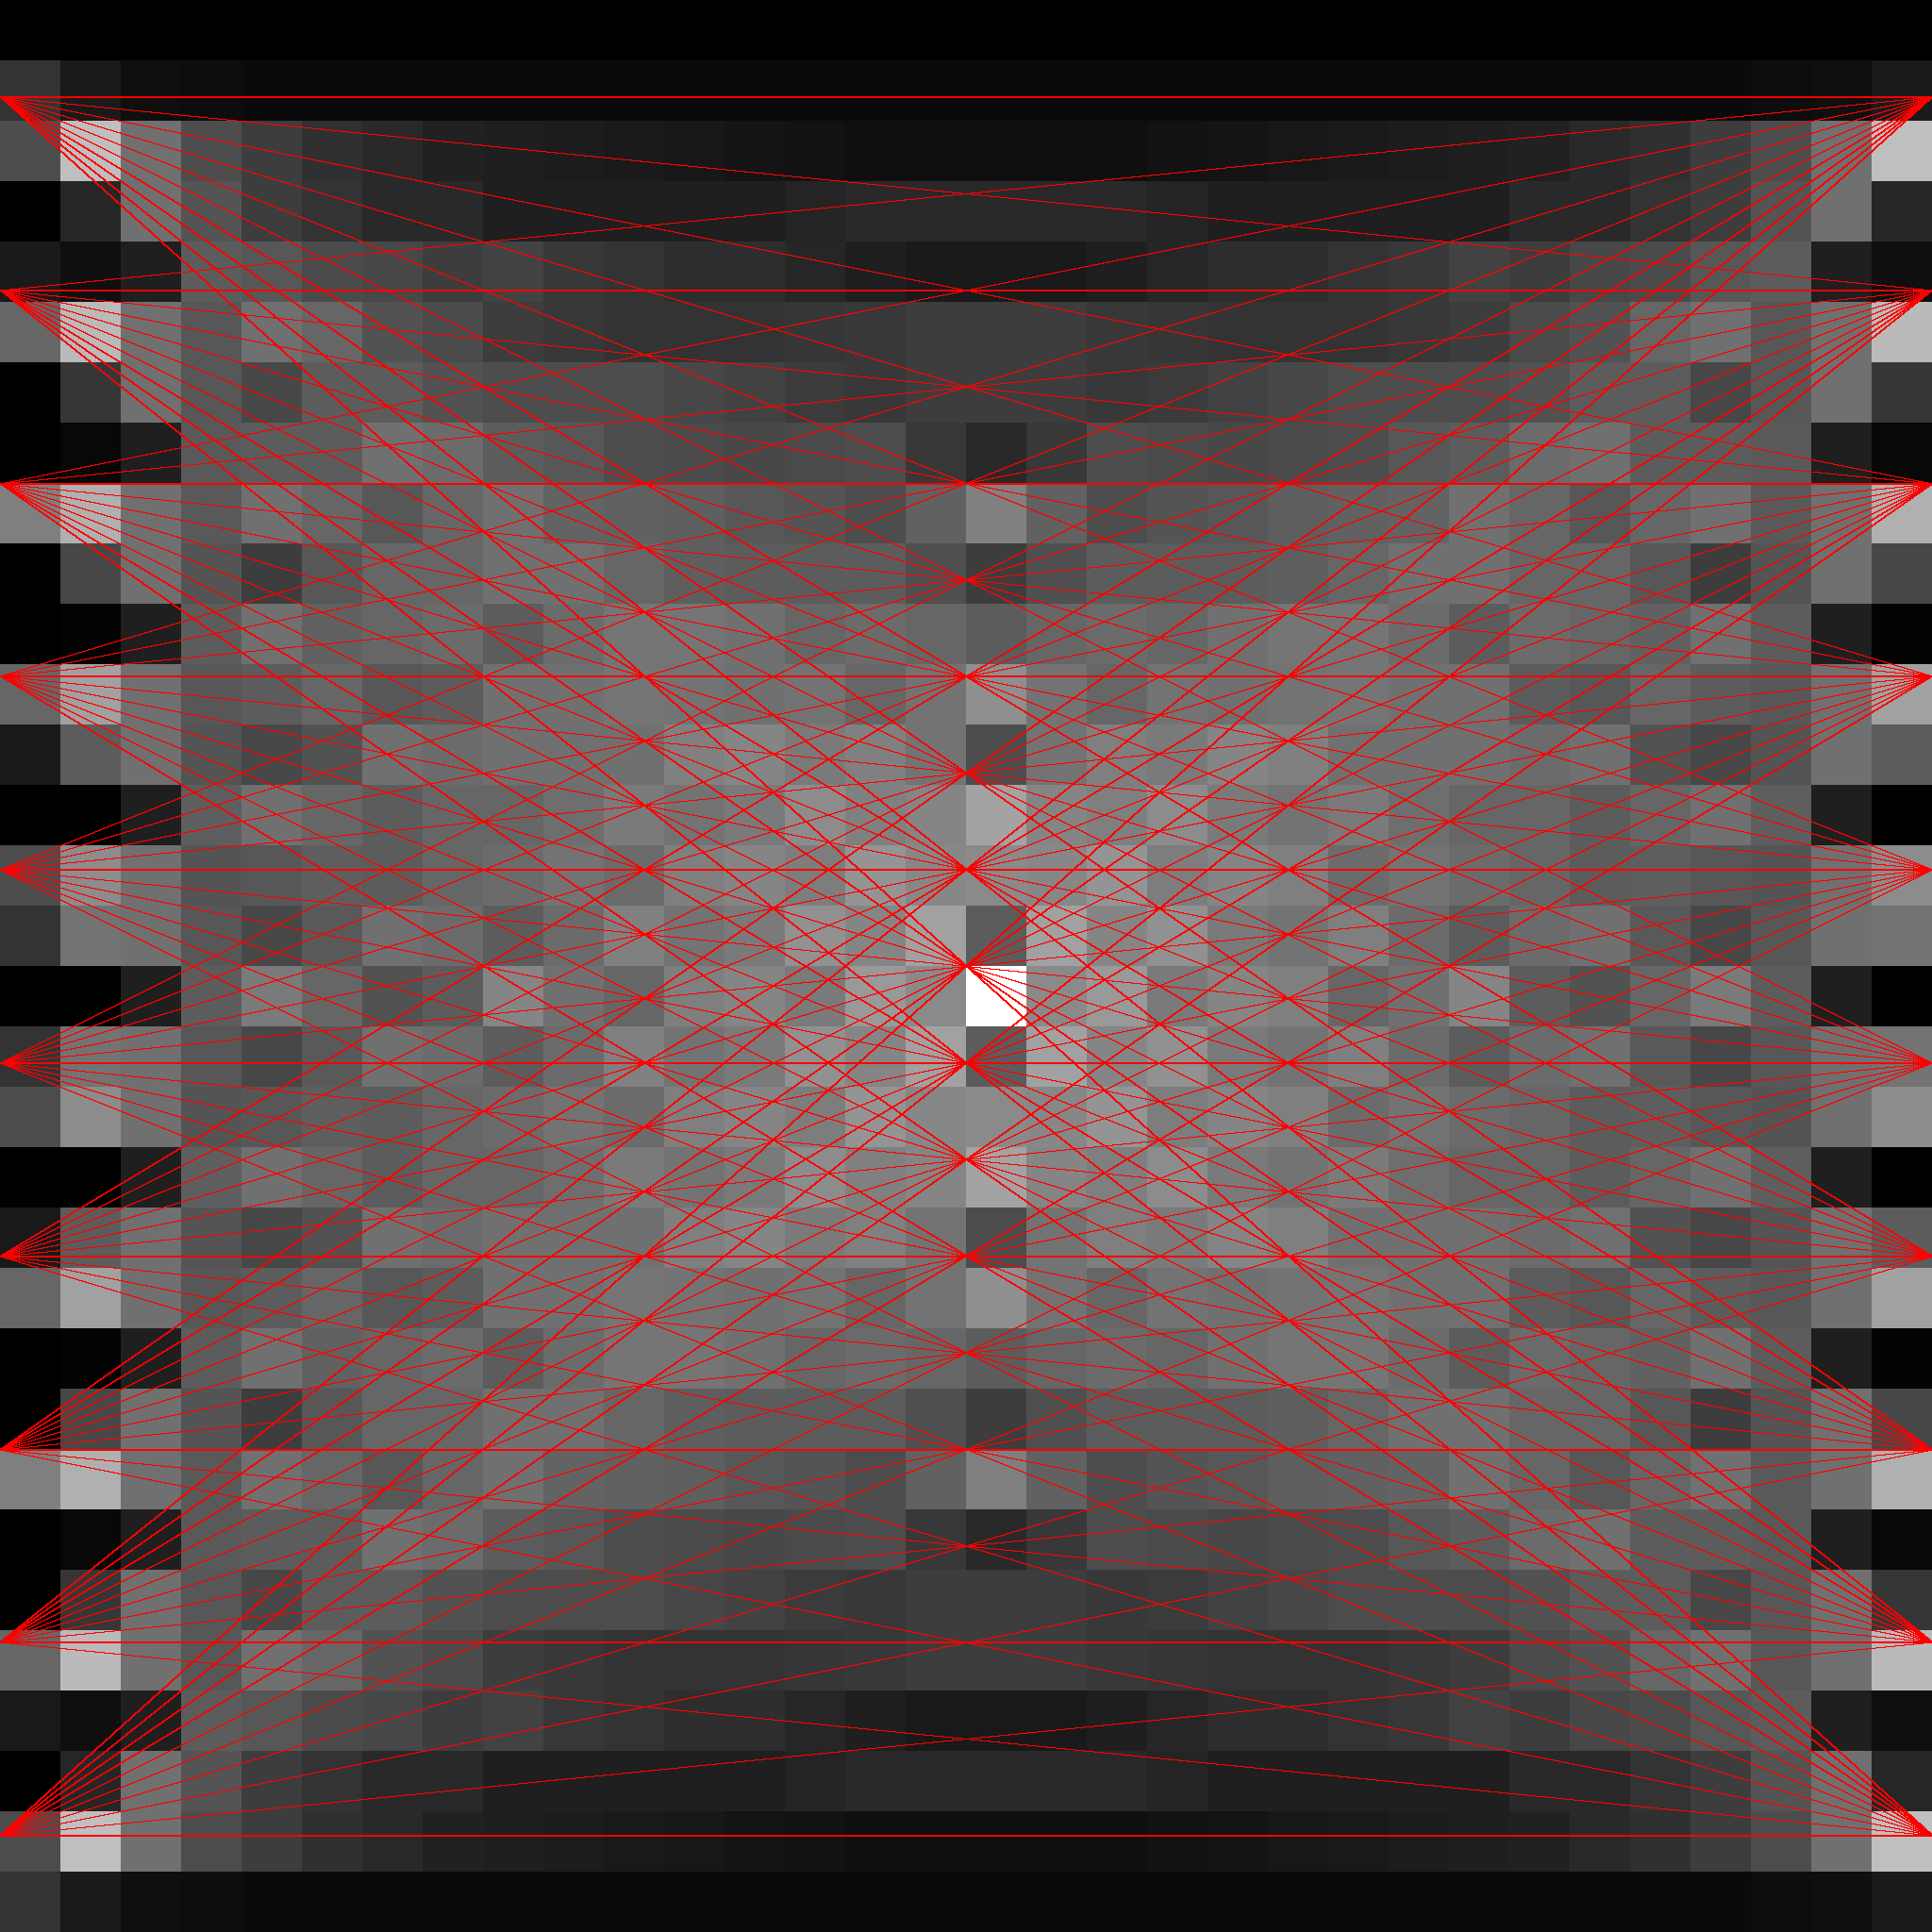
\includegraphics[width=.3\textwidth]{img/exp-anal/raysSides100-heatmap.png} &
    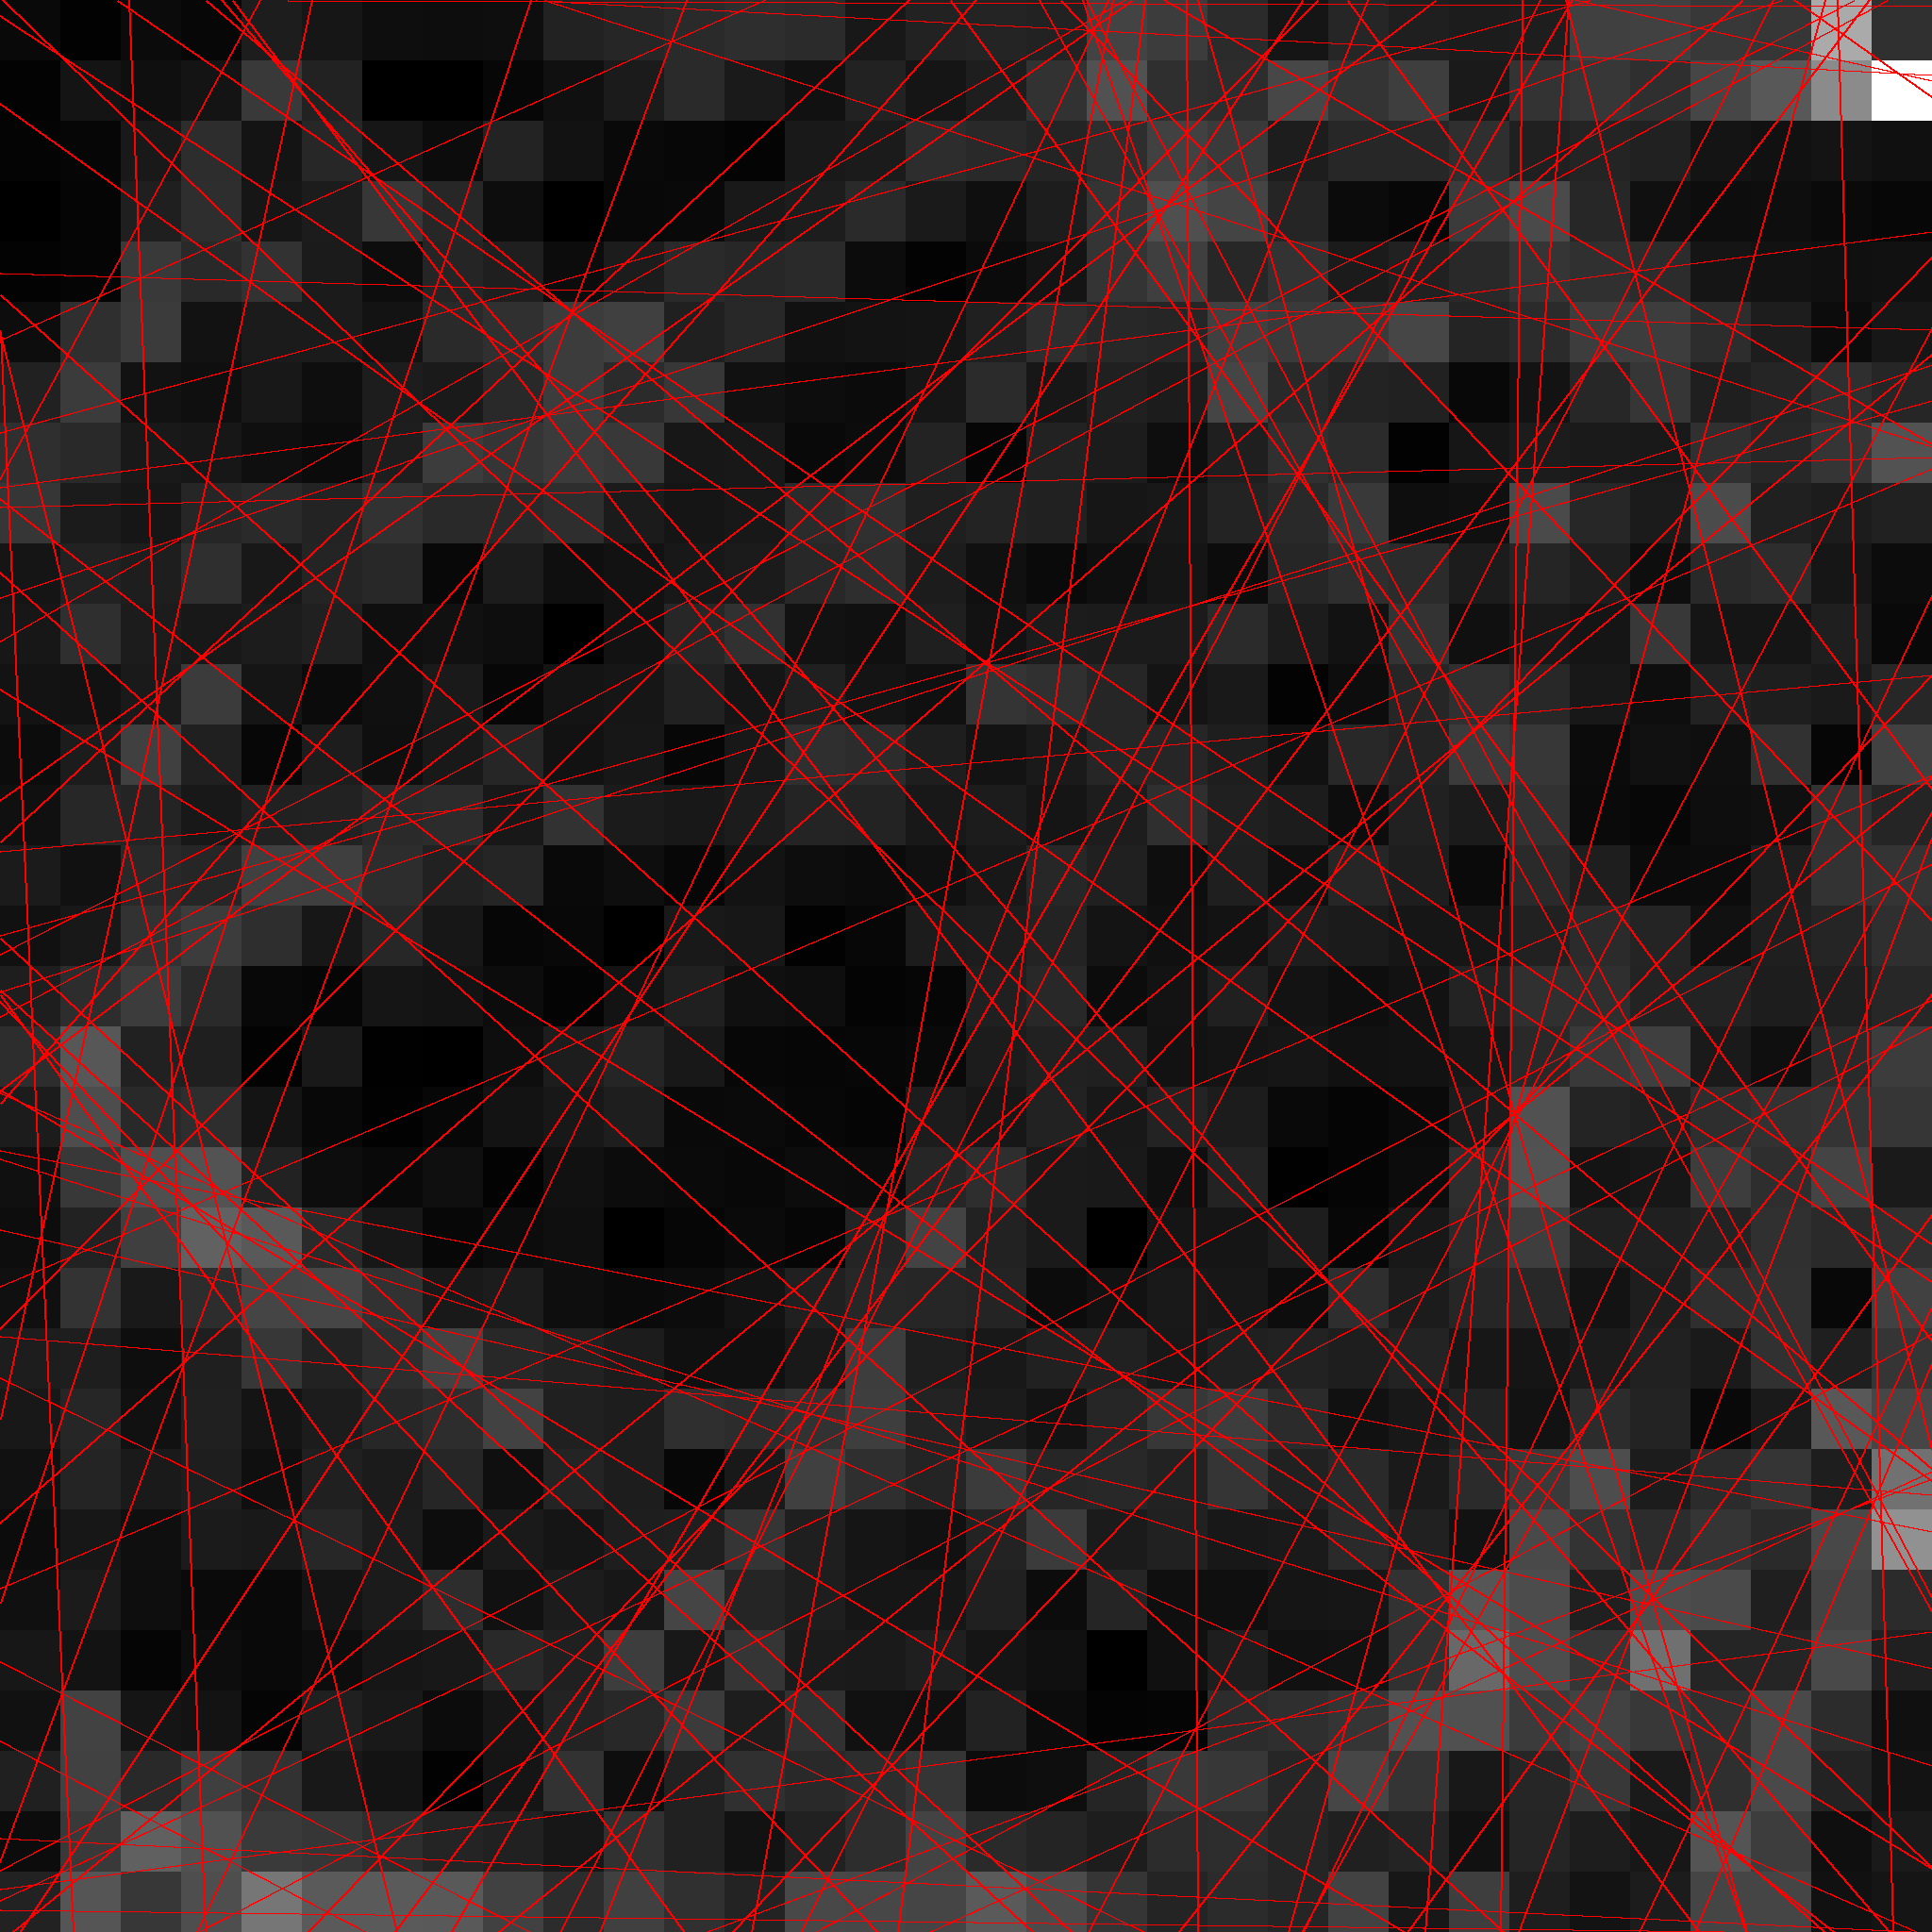
\includegraphics[width=.3\textwidth]{exp-anal/raysRandom100-heatmap.png} & \\
  \end{tabular}
\end{figure}

    % \pnote{- Así se pueden agregar notas para la presentación}
}

\end{document}
